\chapter{Early experiments}

\epigraph{And you may ask yourself \\ "Well\dots how did I get here?"}{Once in a Lifetime \\ Talking Heads, 1981}

In this chapter I showcase early experiments in the different fields I worked on this thesis, with a strong focus on the different aspects of my education and artistic practice.  I include many of my breakthroughs and pitfalls that eventually led me to working on this thesis, in an open, detailed, celebratory, and critical narrative.

\section{Learning microcontrollers}

I learned how to program microcontrollers around 2010 in Chile as an undergraduate student of electrical engineering. I was taught how to program PIC microcontrollers with Microsoft's tools, including the operating system Windows and the C\# programming language. Around the same time, with my classmate Braulio we made our first project with an Arduino Uno microcontroller. It consisted of a robotic guitar tuner, where the Arduino detected the pitch of a string, analyzed the frequency, and then made a servo motor move the tuning gear of the string, in order to match the desired pitch.

\begin{figure}[ht]
  \centering
  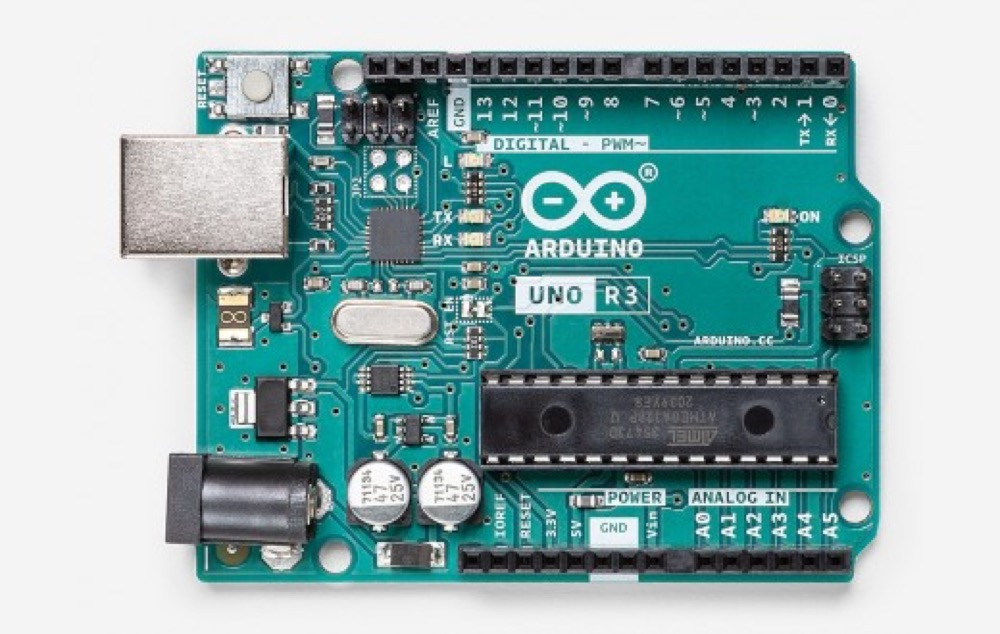
\includegraphics[width=0.75\linewidth,height=0.25\textheight,keepaspectratio]{images/arduino-uno.jpg}
  \caption{Arduino Uno microcontroller}
  \caption*{Retrieved from \cite{website-arduino-uno}}
  \label{fig:arduino-uno}
\end{figure}

Fast forward to 2013, for my undergraduate thesis I had to complete a capstone project and implement many low-level programming techniques, and Arduinos were not allowed because they were considered a shortcut. For this thesis I worked with my classmate Guillermo, and we built a robotic device with a \acrshort{PIC} microcontroller programmed with C\#. Our code was very specific to that particular chip and project, and hardly reusable or interesting for a wider audience.

Since graduation I haven't programmed with \acrshort{PIC} microcontrollers. I realized I wasn't excited about making one-off devices, with non-reusable code that I couldn't share, or having to use propietary or bulky interfaces for writing for deploying my code. In contrast, Arduinos became a huge part of my practice, because of their low cost, open source nature, ease of programming and uploadin the code with a generic USB cable, and because of the enormouus and growing available documentation and user contributed libraries, which now also includie the TinyTrainable library developed for this thesis project.

The Arduino ecosystem fostered many aspects of my practice, and now looking at it in retrospective, it made me realize that what I Love is not computers but computation, making small machines that can crunch numbers for art, and making them openly and in collaboration with friends.

A huge argument that I see people on the internet making against Arduino microcontrollers, is that they are too expensive ( ~30.00 USD) in comparison to the 1/10th of the cost of the bare bones chips and parts you need to build your own microcontroller unit. I am against this argument, since it invisibilizes the effort put in documentation by the Arduino community, and also it assumes that everybody is comfortable soldering and with high advanced electronics degrees. Even if you factor in the cost of hours you need to make your own, it doesn't pay itself. Obviously I see and the educational aspect of building your own things, but it's a slippery slope and discrimination to think that if you build a project with an Arduino it's not good because it's not from scratch, and I think it's rude t say it's not worth it, as rude as yelling at someone buying bread and making fun of them not buying the ingredients and cooking it themselves.

Another strong argument againt Arduino microcontrollers is about efficiency: that Arduino is too high-level and overbloated, and that applications and projects could be faster if you programmed on a lower-level language. I also see this argument when comparing different programming languages for graphic arts. Once again, knowing how to program with lower-level programming languages is amazing, and there is value and fun on it, but in my practice, I put a high value on my time and energy, and I rather make my code slower or less efficient, so I can spend more time making art or resting.

I rather we all have non painful programming experiences, so that we can spend more time away from screens and making art!

\section{Computer music and physical computing}

During undergrad I took classes and did research with professors and computer musicians Rodrigo Cádiz and Patricio de la Cuadra. With them I learned the fundamentals of computer music, including languages such as Max and Pure Data, which I still use to this day. For a class project I created a spoon synthesizer with masking tape, cardboard, and a Makey Makey, a device created in 2021 by Eric Rosenbaum and Jay Silver from MIT Media Lab's Lifelong Kindergarten research group. This was my first hands-on introduction to physical computing, as a way of building my own custom playful interfaces for manipulating sound with computers.
 
\begin{figure}[ht]
  \centering
  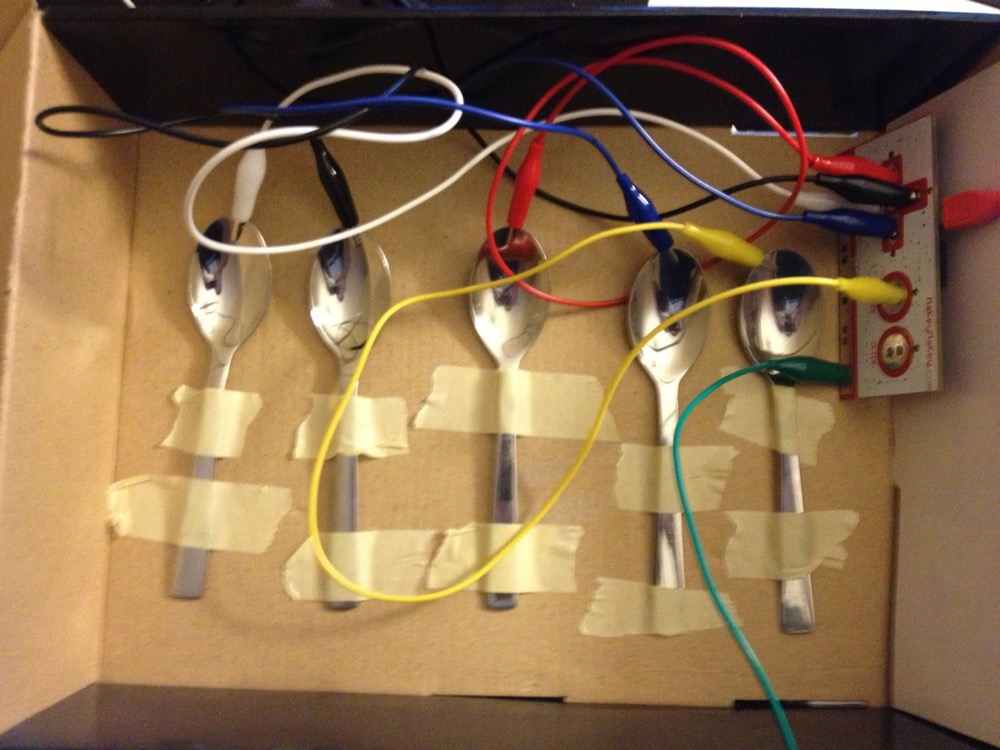
\includegraphics[width=0.75\linewidth,height=0.25\textheight,keepaspectratio]{images/makey-makey-spoons.jpg}
  \caption{Spoons and Makey Makey synthesizer}
  \caption*{Picture taken by myself}
  \label{fig:makey-makey-spoons}
\end{figure}

For this project I applied my practice as a guitar player, where I am constantly mixing and matching different devices on my pedalboard. This inspired me to make this flexible synthesizer with objects lying around me: spoons, masking tape, and cardboard. They also are forgiving, and I was able to change their physical position. The Makey Makey acted as interface with the computer, where I could assign on the fly different sounds to each spae.

In retrospective this project was an instrument an amazing experience that followed Mitchel Resnick's 4 P's: it was a Passion Project that I built for Playing with my Peers, whic is a constant on my artistic practice.

\section{Physical computing and more microcontrollers}

After graduation in 2013 I freelanced as a software and technology designer and developer for artists. I learned computer protocols and networks, and wrote custom software for live multimedia theater and music shows. Realizing that I wanted a bigger community of people to learn media arts with, I applied to New York University's Interactive Telecommunications Program (\acrshort{NYU} \acrshort{ITP}), where I joined as a graduate student in 2015. In my first semester I took the class Introduction to Physical Computing, taught by one of Arduino's co-creators Tom Igoe. Since I was already familiar with electronics and circuits, I focused on learning interface design, human computer interaction, open source hardware and software, and physical computing education.

During my research I was introduced to a wider ecosystem of microcontrollers beyond Arduino, that were possible because of its open source nature and the community behind it. My favorite example is the Teensy by PJRC, which captivated me by two main features: it can send and receive \acrshort{MIDI} over USB, and it has a powerful audio library, that allows you to play audio samples, create effects, and process real time audio. With the Teensy I was able to make standalone projects in a way that before would have required me to use a full fledged computer.

\begin{figure}[ht]
  \centering
  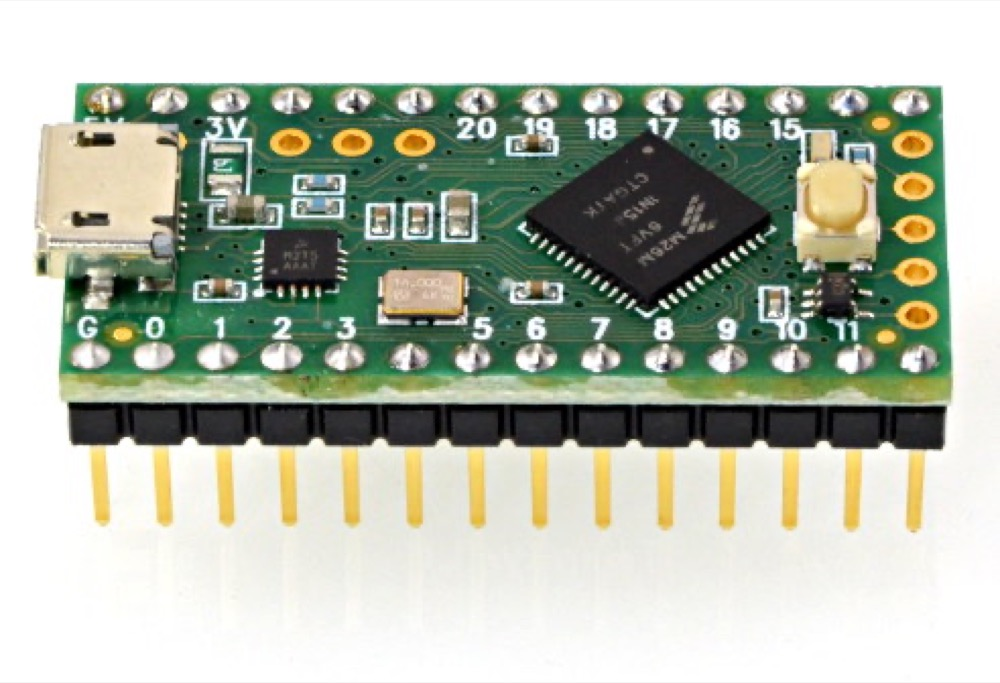
\includegraphics[width=0.75\linewidth,height=0.25\textheight,keepaspectratio]{images/pjrc-teensy-lc-with-pins.jpg}
  \caption{PJRC Teensy LC microcontroller with pins}
  \caption*{Retrieved from \cite{website-pjrc-teensy-lc-with-pins}}
  \label{fig:pjrc-teensy-lc-with-pins}
\end{figure}

\section{Processing and p5.js}

Processing is an open source software written in Java, and it was started at MIT Media Lab's Aesthetics and Computations group by Ben Fry and Casey Reas. Over the years I have learned on my own Processing, and through it computer graphics and interactivity.

I was excited to learn more Processing in 2015 in my first semester at \acrshort{NYU} \acrshort{ITP}'s Introduction to Computational Media class, like it had been taught for around a decade. I consider myself lucky, becasue that year they replaced Processing with p5.js, another software by the Processing Foundation, created by Lauren McCarthy as an inspired port of Processing to JavaScript, to make art that runs on web browsers and over the internet.

I had no experience in web programming, and I hadn't experienced its artistic potential, but I quickly got inspired by web programming. Not only that, Lauren McCarthy was a professor at at \acrshort{NYU} \acrshort{ITP}, and I took her class Performing User \ref{website-nyu-itp-lauren-mccarthy-performing-user}, about performance technology, my favorite class during my master's program.

These educational experiences made me understand better the politic and societal implications of open source softare, appreciate and use the web as an artistic medium, and it inspired my graduate thesis in 2017, a multimedia open source self portrait. This thesis included a piece 

\begin{figure}[ht]
  \centering
  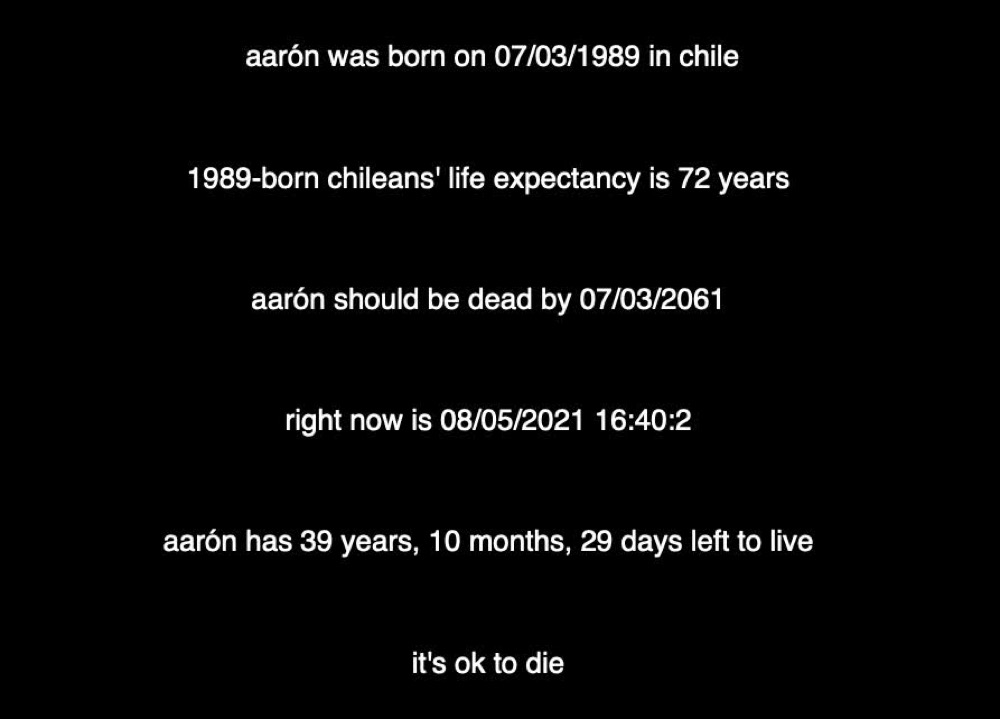
\includegraphics[width=0.75\linewidth,height=0.25\textheight,keepaspectratio]{images/its-ok-to-die-p5js.jpg}
  \caption{PJRC Teensy LC microcontroller with pins}
  \caption*{its-ok-to-die, on a browser with p5.js}
  \label{fig:its-ok-to-die-p5js}
\end{figure}

\begin{figure}[ht]
  \centering
  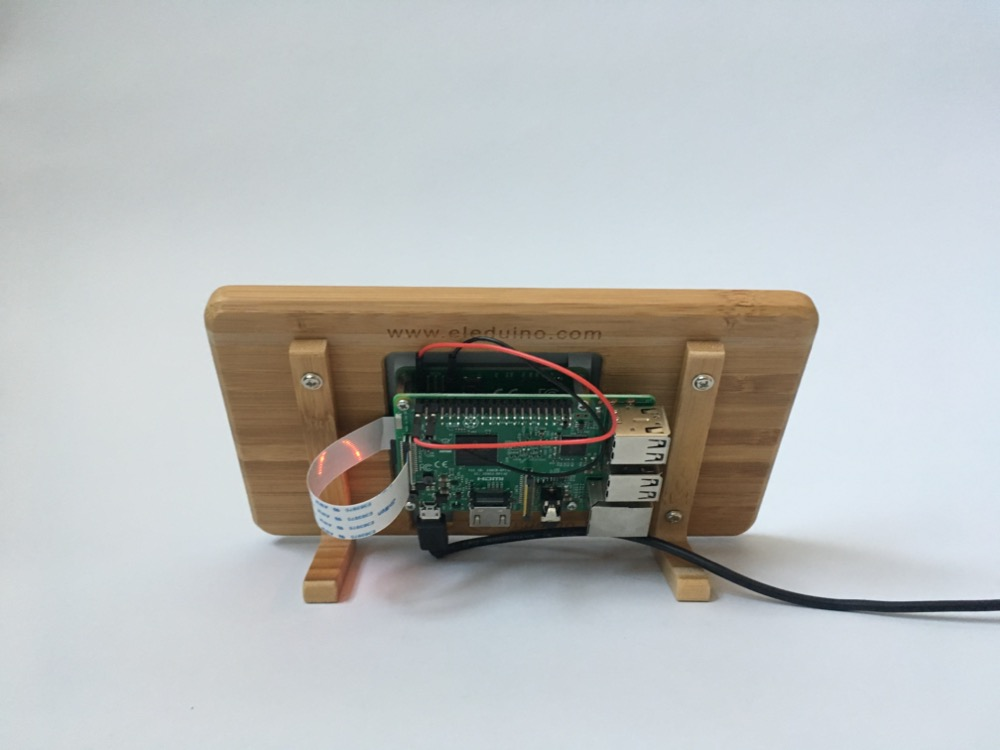
\includegraphics[width=0.75\linewidth,height=0.25\textheight,keepaspectratio]{images/its-ok-to-die-raspberry.jpg}
  \caption{its-ok-to-die, on a Raspberry Pi computer}
  \caption*{Picture taken by myself}
  \label{fig:its-ok-to-die-raspberry}
\end{figure}

At \acrshort{NYU} \acrshort{ITP} I but mostly about web and scripting, and my thesis concentrated on open source, performance art, with only a small hardware component in the form of a Raspberry Pi computer with a countdown timer to my projected death time, according to data by the United Nations, based on my assigned-at-birth-gender and my birth place.

\section{Teaching}

After graduating from \acrshort{NYU} \acrshort{ITP} I focused on media arts education, writing tutorials, teaching introduction to programming workshops for artists.

When I joined MIT Media Lab in 2019, I made the conscious decision of focusing on hardware, to give my creations a life outside of my computer, also inspired by newer restrictive developments by Apple, such as restricting the use of apps created by unregistered developers. In my first semester, which ended up being the only on-campus semester I had, I was introduced by my friend Will Freudenheim to the Shbobo synthesizers by Peter Blasser.

\section{Publishing on the web}

\section{Publishing libraries}

I was partially aware of the instruments made by Peter Blasser, in particular the analog ones.

While at MIT Media Lab, I was delighted by the newer versions of Teensy, which are even faster and more powerful, and which led me to start designing handheld samplers for field recordings, and other standalone devices.

This in turn led me to review the current \acrshort{NYU} \acrshort{ITP} materials for physical computing, where they currently stopped using the now classic Arduino Uno, and have incorporated in their teaching the new series of Arduino Nano microcontrollers, which I based my thesis on.

In particular, the Arduino Nano 33 \acrshort{BLE} Sense I am using, comes with 9 sensors, to measure and detect acceleration, movement, distance, color, and a microphone. This is an amazing breakthrough, since now we can use all this data without having to purchase, install, or calibrate the sensors.

I am using the Arduino's sensors to gather multimedia input data, analyze it with \acrshort{ML}, and then respond with multimedia outputs.

\section{Artistic ML}

My first experiment in this field was with my \acrshort{NYU} \acrshort{ITP} classmate Corbin Ordel, who was a student at Gene Kogan's \acrshort{ML} for Artist class. Together we audited Rebecca Fiebrink's \acrshort{ML} for Musicians and Artists class, available at the Kadenze platform, and learned the Wekinator platform.

Our project is Piano Die Hard, a digital sculpture consisting on a piano that reacted in real time, 


teamed up to hack a project we called Piano Die Hard, built with open source tools such as Wekinator, Arduino, openFrameworks, and using the \acrshort{ML} algorithm KNN. We created a video database of explosions in the Die Hard movie franchise, and another one of other 1980's movies with no explosions, and we trained our \acrshort{ML} algorithm to distinguish between the categories explosion and no explosion. We featured this project at a \acrshort{NYU} \acrshort{ITP} show, were written up at the Daily Beast newspaper, and exhibited our work at the alt-ai conference.

In 2017, while I was finishing my appointment as research resident at \acrshort{NYU} ITP, Cristóbal Valenzuela had started the project RunwayML as his master's thesis, which is now a company led by Cristóbal, Alejandro Matamala and Anastasis Germanidis.

At \acrshort{NYU} \acrshort{ITP} I also saw the first experiments with deeplearn.js, later TensorFlow.js, which soon became the foundation of the ml5.js library, a wrapper for TensorFlow.js, for on-the-browser \acrshort{ML}.

I decided I wanted to dip my toes in \acrshort{ML}, so I took a month-long intensive class at the School of Machines in Berlin, Germany, facilitated by Gene Kogan and Andreas Refsgaard, and organized by Rachel Uwa.


A big inspiration for this thesis has been the book on GANs by Casey Reas, published by Anteism, as of 2021 on its second edition. It’s an arts-first book that contextualizes the use of \acrshort{ML} algorithms for the creation of images, and uses the metaphor of these algorithms as being similar to the development of the camera. Artists don’t need to understand all the physics or mechanics behind a camera in order to make art with it, but it can help to understand it too. I think \acrshort{ML} is also a game changer for instrument making, and \acrshort{ML} introduces new civic complexities, and my thesis tries to follow the example of this book, to introduce the technology and contextualize for a new generation of artists and instrument makers.

Since many \acrshort{ML} projects rely on proprietary hardware, such as NVIDIA GPUs, or rely on the cloud for faster compilation times, for this thesis I decided to make open source \acrshort{ML} projects that people could read and understand and remix and hack.

TODO: mention the impact of the documentary Coded Bias, and how these researchers impacted my desire to make my thesis. Also mention how right before pandemic I had started a pottery class, with the intention of making clay-based instruments for thesis, as a metaphor of making code and hardware and software feel fluid and not static, I want to empower people to program, in particular \acrshort{ML} because of its dangerous implementations by oppressive governments and corporations, and in particular for arts, for making artists dream come true.
